\documentclass[journal]{vgtc}                % final (journal style)
%\documentclass[review,journal]{vgtc}         % review (journal style)
%\documentclass[widereview]{vgtc}             % wide-spaced review
%\documentclass[preprint,journal]{vgtc}       % preprint (journal style)
%\documentclass[electronic,journal]{vgtc}     % electronic version, journal

\let\ifpdf\relax

%% Uncomment one of the lines above depending on where your paper is
%% in the conference process. ``review'' and ``widereview'' are for review
%% submission, ``preprint'' is for pre-publication, and the final version
%% doesn't use a specific qualifier. Further, ``electronic'' includes
%% hyperreferences for more convenient online viewing.

%% Please use one of the ``review'' options in combination with the
%% assigned online id (see below) ONLY if your paper uses a double blind
%% review process. Some conferences, like IEEE Vis and InfoVis, have NOT
%% in the past.

%% Please note that the use of figures is not permitted on the first page
%% of the journal version.  Figures should begin on the second page and be
%% in CMYK or Grey scale format, otherwise, colour shifting may occur
%% during the printing process.  Papers submitted with figures on the
%% first page will be refused.

%% These three lines bring in essential packages: ``mathptmx'' for Type 1
%% typefaces, ``graphicx'' for inclusion of EPS figures. and ``times''
%% for proper handling of the times font family.

\usepackage{mathptmx}
\usepackage{graphicx}
\usepackage{times}

\usepackage{pbox}

%% We encourage the use of mathptmx for consistent usage of times font
%% throughout the proceedings. However, if you encounter conflicts
%% with other math-related packages, you may want to disable it.

%% If you are submitting a paper to a conference for review with a double
%% blind reviewing process, please replace the value ``0'' below with your
%% OnlineID. Otherwise, you may safely leave it at ``0''.
\onlineid{0}

%% declare the category of your paper, only shown in review mode
\vgtccategory{Research}

%% allow for this line if you want the electronic option to work properly
\vgtcinsertpkg

%% In preprint mode you may define your own headline.
%\preprinttext{To appear in an IEEE VGTC sponsored conference.}

%% Paper title.

\title{The impact of user interface design of eco-feedback systems on consumer behavior}

%% This is how authors are specified in the journal style

%% indicate IEEE Member or Student Member in form indicated below
\author{Aur\'{e}lie Fakambi and Wouter Menninga}
\authorfooter{
%% insert punctuation at end of each item
\item
  A. Fakambi is a Computing Science Master student at the University of Groningen, E-mail: A.Fakambi@student.rug.nl.
\item
  W. Menninga is a Computing Science Master student at the University of Groningen, E-mail: W.G.Menninga@student.rug.nl.
}

%% A teaser figure is NOT to be included.

%other entries to be set up for journal
%\shortauthortitle{Biv \MakeLowercase{\textit{et al.}}: Global Illumination for Fun and Profit}
%\shortauthortitle{Firstauthor \MakeLowercase{\textit{et al.}}: Paper Title}

%% Abstract section.
\abstract{Saving energy in buildings ad homes has become and remains a major issue for the planet.
It avoids waste of irreplaceable sources of energy and decreases pollution and at the same time help the companies and household saving money, everyone can benefit from reducing their energy consumption.
For this purpose during the last decade, systems have been developed to provide consumers with information about their energy consumption. 
Research has shown that the type of information displayed and the techniques used to present it have an impact on the user energy saving. This raises the question about how to display the information to the consumer in a comprehensive, attractive and non-intrusive way. \\

In this paper, we compare and discuss the various methods of visualizing energy usage for consumers. Some of the design components of user interfaces such as historical comparisons and presentation of costs are more likely to aid in providing the consumer with an understanding of his energy usage and changing his behavior.
We will extract the most effective methods from research and surveys. \\

The comparison of the different methods is based on results achieved in previous studies, namely the reduction of energy usage of consumers using such eco-feedback systems and the answers by such users to questions in surveys.\\

Little work has been done in the design of eco-feedback systems. However, the researchers in the domain (Human Computer Interface designers and environmental psychologists) agree that components such as historical comparison, presentation of costs and disaggregation by appliance are the most effective ones, even though there are no universal rules because the context is also really important.
 %We expect to find the most effective methods to visualize energy consumption data for future eco-feedback systems.

} 

%% Keywords that describe your work. Will show as 'Index Terms' in journal
%% please capitalize first letter and insert punctuation after last keyword
\keywords{Eco-Feedback, interface design, energy consumption, consumption feedback systems, energy feedback. Human Computer Interfaces}

%% ACM Computing Classification System (CCS). 
%% See <http://www.acm.org/class/1998/> for details.
%% The ``\CCScat'' command takes four arguments.

\CCScatlist{ % not used in journal version
  \CCScat{K.6.1}{Management of Computing and Information Systems}%
{Project and People Management}{Life Cycle};
  \CCScat{K.7.m}{The Computing Profession}{Miscellaneous}{Ethics}
}

\manuscriptnote{~}

%% Copyright space is enabled by default as required by guidelines.
%% It is disabled by the 'review' option or via the following command:
% \nocopyrightspace

%%%%%%%%%%%%%%%%%%%%%%%%%%%%%%%%%%%%%%%%%%%%%%%%%%%%%%%%%%%%%%%%
%%%%%%%%%%%%%%%%%%%%%% START OF THE PAPER %%%%%%%%%%%%%%%%%%%%%%
%%%%%%%%%%%%%%%%%%%%%%%%%%%%%%%%%%%%%%%%%%%%%%%%%%%%%%%%%%%%%%%%%

\begin{document}

%% The ``\maketitle'' command must be the first command after the
%% ``\begin{document}'' command. It prepares and prints the title block.

%% the only exception to this rule is the \firstsection command
\firstsection{Introduction}

\maketitle

%% \section{Introduction} %for journal use above \firstsection{..} instead

% problem of energy usage
Reducing energy usage in buildings and homes still remains a major challenge. It would lead to a better environment with less pollution and waste of energy. The consumers could also save money if they adopted a more sustainable and energy efficient behavior. % we can develop
One method to reduce energy consumption is by increasing the awareness of consumers about their energy consumption using eco-feedback systems. These are systems with integrated sensors that provide the consumers in the building with information about their energy usage. The goal is that this leads to more energy efficient behavior by the consumers in the building. 

However, research has shown that the types of information displayed and the techniques used to present it have an impact on the user behavior.
For example, studies have demonstrated that the information provided must be intuitive, clear and simple and the UI attractive and not too intrusive (e.g. not too many notifications) so that the users keep using it and is integrated in their everyday life \cite{spagnolli2011eco}.

This means that the design of the user interface is a key factor in changing the user energy consumption behavior of the user and raises the question of what the most effective methods to visualize energy consumption data for future eco-feedback systems are. 

% to be corrected ?
Our goal is to investigate the different ways to display to the users their electricity usage.
% REFERENCE
% Assessing eco-feedback interface usage and design to drive energy efficiency in buildings
% Consumer preferences for feedback on household electricity consumption
Researches and developers have selected %agree to say that
the main design components of eco-feedback systems % REFERENCES THERE
: presentation of costs, historical comparison, incentives, disaggregation by appliance and goal setting. From those components we want to extract the most effective ones, the ones which are more likely to help users saving energy. 


% to be corrected ?
Based on previous surveys we are going to compare the effectiveness of different eco-feedback systems by comparing the reduction in electricity usage. %provoked by the usage of such or such component OR when using such or such design component
Additionally, we will combine the results and responses of surveys and interviews with users of such eco-feedback systems, to assess the effectiveness of different UI components. \\

% AURELIE COMMENT , rephrase:
We aim at answering many questions in our paper, related to the many decisions that have to be made when designing eco-feedback systems: \textbf{what type of data} should be displayed? and\textbf{how and how much} should the data be displayed to users? 
%\begin{itemize}
%\item \textbf{what type of data} should be displayed? 
%\item \textbf{how and how much} should the data be displayed to users? 
%\end{itemize}
% methode
%For this comparative paper, we made a selection out of the previous work. 

In the first part of this paper the design components will be presented. In the second part, the surveys and studies will be elaborated on and in the third part we will present the results based on these studies and surveys. % To be improved

%to find the most effective methods to visualize energy consumption data for future eco-feedback systems.

% 'integrating sensors and systems to create eco feedback systems' which provide people in building with information about energy consumption behavior 
% many studies have shown that feedback works effectively...[ref]
%It has been shown in many studies that feedback systems have effect in reducing energy consumption
% design of user interface is a key factor to have impact on energy behavior
\section{Eco-Feedback System Design}
Developers have been implementing different types of applications: classical eco-feedback systems or serious games (e.g. games which the purpose is not just entertainment) %( ex *** ) 
to make it even more attractive to the users and increase their commitment.

Important aspects of eco-feedback systems are the kind of information displayed and the method of display. However, the aesthetics are also relevant for the engagement, pleasure and interest of the user \cite{bartram2015design}.

In most of the eco-feedback systems some design components are often encountered.
In this part they will be defined and later we will discuss their effect on users changing behavior in order to elect the most effective ones. 

%\subsection{Displays}
%Eco-feedback systems are available on smart meters, personal computers, mobile devices and house/wall displays. %TODO what is better?? 
% AURELIE COMMENT : should we have a part only for the displays

\subsection{User Interface Components}
The following sections describe the different UI components often used in the design of eco-feedback (ECF)systems.
\subsubsection{Consumption over time}
The \textit{consumption over time} UI component is one of the most basic components. It simply displays the consumption of energy over time. Usually, several time scales can be selected, like the last few hours, days or weeks.
Almost all eco-feedback systems have a component like this one \cite{spagnolli2011eco}. 
An example can be seen at 4 in Figure~\ref{fig:electricityportal}.

\subsubsection{Historical \& Normative comparison}
Two types of comparison are often presented in eco-feedback systems: historical and normative.\\

\textit{Historical comparison} is defined as the ability of users to view their current consumption compared to their past consumption. %SOURCE
The historical comparison can often be displayed on a daily, weekly, monthly or yearly basis. It is used in the majority of eco-feedback systems, because it can be easily understood by the users, especially thanks to the use of bar charts. %(cf part BLABLABLA).
Observing those graphs helps reminding users of their behavior (why they used more energy this particular day for example) and in consequence aids in changing their bad habits.

Most eco-feedback systems do not take into account factors such as weather (more energy is used when it is colder) or households leaving for vacation when establishing the historical comparison \cite{karjalainen2011consumer}. This means that absolute values are analyzed whereas they should have been normalized first. Some improvements in the eco-feedback systems take those fluctuations and changes into account for more accuracy and consistency. \\

%The historical comparison deals with comparison with the household's own prior consumption 
Another type of comparison is the \textit{normative comparison}, which deals with comparison at a local, regional level or in a neighborhood. The effectiveness of the normative comparison comes from the fact that users are influenced by social norms and pressure. Seeing, for example, that their neighbors consume less energy than they do, should encourage them to do the same. It has been seen in previous research that such normative comparisons can lead to significant reductions in electricity usage \cite{peschiera2010response,siero1996changing,iyer2006comparison}.

%We will see in the Survey section that the historical comparison is the most effective one.

\subsubsection{Incentives}
\textit{Incentives} (rewards and penalization) allow users to earn rewards if they reduce their energy consumption or on the contrary to be penalized if they waste energy. The idea is that a system of rewards and penalization encourages behavior that leads to energy conservation and discourages wasteful behavior.

The incentive design component is strongly related to the rewards \& penalization design components. Users can be rewarded in a financial or non-financial way. Financial incentives can be, for example, credit on an electricity bill and non-financial incentives can be prizes such as an energy efficient lamp or reaching higher levels in the game.
Previous research \cite{petersen2007dormitory} has shown that incentives can result in significant reductions of the electricity consumption.

\subsubsection{Disaggregation or appliance specific breakdown}
\textit{Disaggregation} or appliance-specific breakdown allows consumers to have a better understanding about which appliance consumes what, so it is easier for them to change a particular behavior. It helps consumers to understand the impact of the use of an appliance to answer questions like: ``if I let the TV on for 5 hours, how much do I consume?".
We'll see in the survey part with some examples of UI that this deisgn component is often presented with pie charts most of the time and also with bar charts.
%However this design component is C'est toujours à l'étape de recherche because installing and maintaining individual sensors is difficult.

\subsubsection{Goal setting}
Environmental psychology departments have demonstrated that users need to find motivation in order to change their behavior \cite{abrahamse2007effect}.
Some eco-feedback systems provide \textit{goal setting} design components: the users can set the goal themselves or they are pre-configured by the software or set by the community of users of the eco-feedback system.  %AURELIE new :
One way to generate a goal setting is to compute a baseline of energy consumption based on past usage and then set the goal as some percentage reduction from the baseline. % the computation of this baseline won't be presented in here
An example of a goal could be: ``reduce your energy consumption with 5\% compared to the previous month''.

Every household consumes in a different way. Therefore, households in the same neighborhood are not likely to have the same goals.
Eco-feedback systems can aid users to reach their goal thanks to tips and advices.
To motivate the users, the eco-feedback system should reward them when they reach their goal. 



\subsection{Presentation of the information inside the components} % Neeeed a better title
% Description

%In this section different ways to present information will be described.
% the ''how'' question is answered there
What is the best and most effective way to present the information inside the key design components identified in the previous part? What do the users understand easily: texts or graphs?

Developers have several options to present the same information: text, graphs, pie and bar charts, tables etc.

Moreover, the choice of colors is also really important. There should not be too many colors so that the UI stays pleasant for the eye and the designers should not use the same colors to display different kinds of information.

\subsubsection{Choice of units for numerical data}
The data provided to the users has to be understandable and familiar. The designers can present the energy consumption with scientific units such as: kWh (usually used in the bill), kg CO2, Joule or using a monetary unit, like euros or environmental units such as trees saved.
To make it attractive for users, some designers do not lack in originality in their choice of units for displaying the amount of consumed energy. For example, an exposition in the Bernoulliborg by ScienceLinX shows an Eco =-Feedback System (ECF) which displays the consumption in the units ‘hamburgers or coffees bought’.
%Kind of presentation that the users prefere graphical vs Text => guidelines of Smith and Mosier
%More information about the chart pie, bar chart, tabular presentation understanding among users.

%\subsection{Colors}
%From the surveys and studies the most powerful will arise.

\section{The Surveys and Studies}
Several studies researching the effectiveness of consumer feedback on electricity consumption have been done before.
This section will describe a selection of those studies and analyze the results.
The studies can be divided into two components: a user wishes component and a comparative component.
% Why did we select those surveys ? Advantages, disadvantages BLABLABLA
We selected a wide range of surveys :some of them are theorical, while others are made in real situations or with real and availavle protoypes. Using different methods and approaches will allow us to have a better insight and a user-centered approach.

\subsection{User wishes surveys}
Several past studies have done a user wishes survey, exploring the opinions of users (generally household consumers) by asking them a set of questions. 
% Interviews
User wishes surveys are really interesting because who else than the users know what is good for them ? It allows the researchers and developers to really understand what can affect and impact the user behavior.

\subsubsection{Survey by Karjalainen}
In a study from S. Karjalainen \cite{karjalainen2011consumer} from 2010, interviewing was used to find the best ways to present information for maximum energy reductions. In this study, interviews with consumers were held to find out about their attitude towards energy monitoring and what kind of feedback they understand and prefer.

The qualitative interviews showed that 8 out of 14 interviewees actively try to save electricity at home, while all 14 responded they want to monitor electricity consumption. The interviewees also indicated that they prefer to receive feedback via a bill, web page or dedicated wall display rather than a mobile phone.

Participants were also asked some general questions about how important they find certain aspects of eco-feedback systems. The questions were answered using a scale of 1 to 5, where 5 was very important and 1 not important at all. The questions, along with the average of the response of the 14 participants, can be seen in Table~\ref{prototypesquestions}.

% results
\begin{table}
%% Table captions on top in journal version
  \caption{General questions about eco-feedback systems  \cite{karjalainen2011consumer}}
  \label{prototypesquestions}
  \scriptsize
  \begin{center}
    \begin{tabular}{|ll|}
    \hline
       Question (\textit{How important is it to...}) & Avg. \\ \hline
       \pbox{20cm}{\textit{be able to compare your household's consumption}\\\textit{to other households?}} & 3.6 \\ ~\\[-0.25cm]
       \textit{be able to compare your consumption to your prior consumption?} & 4.4 \\ 
       \textit{have a target level for consumption?} & 3.5 \\ 
       \textit{know the consumption of individual devices?} & 4.1 \\ 
       \textit{receive information on actions which would save energy?} & 3.9 \\
       \hline
    \end{tabular}
  \end{center}
\end{table}
% OUR OWN SURVEY

\subsubsection{Own Survey}

In order to have more insight/more information about what young potential users want, we conducted a survey\footnote{Results are available online at {http://goo.gl/eoUUoD}} that we posted on social networks: Facebook and Twitter.
The 31 respondents were aged from 16 to 26.%\footnote{The results are available online at \url{}}
% MOTIVATION 
We decided to target young people because it could be more efficient. Our hypothesis is that it's problably easier for them to change their bad habits compared to adults. Moreover we could take advantage of the relation between them and technology. They are really familiar with apps and use really often their smartphones so there is an opportunity for developers to build apps and games especially for them.Therefore this approach is new compared to the ones you will read in this paper and the one present in the litterature.

First, we learnt that most of the participants (55\%) want to save energy, but do not know how to accomplish this and also that a lot of respondents are unaware of the existence of eco-feedback systems (65\%).
 
Not surprisingly, young people want an app (80\%) which could either be a classical ECF system (45\%) or a game (55\%).
They prefer graphs such as pie charts and bar charts (88\%), rather than text or tables. 
Moreover, compared to historical comparison and presentation of costs, disaggregation by appliance (52\%) is favoured by the participants.
When asked if they would be more motivated to save energy if they knew how much energy their peers use, about half of them (48\%) replied that they did not mind and the other half of them said it would motivate them.
The respondents indicated that money is the most understandable unit for them (77\%), while scientific units like kg of CO$_2$ were indicated to be less understandable.

In the next part we will see if the other studies and their outcomes are consistent with the results of this one.



\subsection{Comparison/comparative surveys} %better title to be found
Studies in the past have also collected data about energy consumer behavior in response to several different eco-feedback systems. These eco-feedback systems have different UI components and can therefore be used for a comparative analysis.

\subsubsection{Karjalainen}
In the study from S. Karjalainen \cite{karjalainen2011consumer}, 8 paper user interface prototypes were developed. Table~\ref{prototypes} shows an overview of the UI components present in these prototypes.

\begin{table}[h]
%% Table captions on top in journal version
  \caption{Overview of information presented in the different prototypes by Karjalainen \cite{karjalainen2011consumer}}
  \label{prototypes}
  \scriptsize
  \begin{center}
    \begin{tabular}{r|cccccccc}
    
      \multicolumn{1}{c|}{UI component} & \multicolumn{8}{c}{Prototype} \\
    
       & 1 & 2 & 3 & 4 & 5 & 6 & 7 & 8 \\
    \hline
      Historical comparison & $\times$ &  &  &  &  &  &  & \\ \hline
      Normative comparison &  & $\times$ & $\times$ &  &  &  &  & \\ \hline
      Goal setting &  & $\times$ &  &  &  &  &  & \\ \hline
      Consumption (kWh) & $\times$ & $\times$ &  &  &  & $\times$ & $\times$ & $\times$ \\ \hline
      Power (W) &  &  &  & $\times$ & $\times$ &  &  & \\ \hline
      Costs (Euro) &  & $\times$ &  &  &  & $\times$ &  & \\ \hline
      Environmental factor (kg CO$_2$) &  &  & $\times$ &  &  &  &  & \\ \hline
      Household total & $\times$ & $\times$ & $\times$ & $\times$ & $\times$ & $\times$ & $\times$ & \\ \hline
      Disaggregation day/night &  &  &  &  &  &  & $\times$ & \\ \hline
      Disaggregation by device &  &  &  &  & $\times$ & $\times$ & $\times$ & $\times$ \\ \hline
      Chart & $\times$ &  &  & $\times$ & $\times$ &  & $\times$ & $\times$ \\ \hline
      Table &  &  &  &  &  & $\times$ &  & \\ \hline
      Other numeric &  & $\times$ & $\times$ &  & $\times$ &  &  & $\times$ \\ \hline
      Textual &  &  & $\times$ &  &  &  &  & \\ 
    \end{tabular}
  \end{center}
\end{table}

The prototypes were shown to consumers one by one and after showing all the prototypes, they were asked if they understood the prototypes and asked to choose the prototype they would prefer to use themselves.

The results of the survey can be seen in Table~\ref{prototypesresults}. Most prototypes were understood by the participants. From the results in this table, when combined with the definitions of the prototypes in Table~\ref{prototypes} ,we can conclude that components such as: consumption in kWh, presentation of costs, disaggregation by device and table are features/components which are easy for the users to understand. Problems with understanding were mostly due to the fact that many people are not familiar with the scientific units used and do not, for example, understand the difference between W and kWh. Secondly, people in general do not understand how CO$_2$ emissions relate to energy consumption.
In contrast, information presented in charts and tables is understood easily by the participants.

We can conclude that presentation with measures such as kgCO2 and text are not helpful and difficult to understand for the users.


% results
\begin{table}
%% Table captions on top in journal version
  \caption{Nr of participants that understood and preferred for each of the prototypes. Total participants: 14. \cite{karjalainen2011consumer}}
  \label{prototypesresults}
  \scriptsize
  \begin{center}
    \begin{tabular}{|lcc|}
    \hline
       & \multicolumn{1}{p{2.5cm}}{\centering Nr of participants that understood prototype} & 
       \multicolumn{1}{p{3cm}|}{\centering Nr of participants who preferred prototype}  \\ \hline
       Prototype 1 & 14 & 1 \\ 
       Prototype 2 & 14 & 1 \\ 
       Prototype 3 & 8 & 0 \\ 
       Prototype 4 & 12 & 0 \\ 
       Prototype 5 & 7 & 1 \\ 
       Prototype 6 & 14 & 7 \\ 
       Prototype 7 & 13 & 1 \\ 
       Prototype 8 & 14 & 3 \\ \hline
    \end{tabular}
  \end{center}
\end{table}

The results of this study by Karjalainen found the following UI components most valued by consumers: presentation of costs, device-specific breakdown of energy usage and historical comparison.  % TODO: why?

\subsubsection{Peschiera et al.}
Research from 2010 by Peschiera et al. \cite{peschiera2010response} provides more insight into the effectiveness of the normative comparison component. In their study, they tried to find out if there are differences in energy savings when participants only view personal electricity usage information versus participants also viewing average building occupant usage and usage of peers in their personal network.

%FIXME: the following part is too 'narrative' and 'detailed'
To examine if such normalized comparison information motivates electricity-saving behavior, they fitted 83 rooms of a dormitory building in New York City to measure the electricity usage.

They divided the occupants participating in the study into four distinct groups:
\begin{itemize}
\item \textit{Group A} -- ability to view individual historical comparison with past vs. present utilization.
\item \textit{Group B} -- same as group A, but with additional ability to view individual vs. average electricity usage of all other participating occupants.
\item \textit{Group C} -- same as group B, but with additional ability to view electricity usage of peers in that individual's network.
\item \textit{Control Group} -- No access to electricity usage information.
\end{itemize}

%At the start of the study, occupants received an email explaining how to access their personal electricity consumption reports. During the study, they received several more notification emails to remind them that their electricity usage report was ready.

Three days after the start of the study, the average electricity consumption for Group C was 34\% lower than the consumption of the Control Group and 20\% lower than the consumption in the period before the study.
After sending the second consumption notification email, the average electricity consumption dropped to 45\% below that of the Control Group (28\% less than before the study).
Group B only saw a significant reduction after the second notification email and Group A did not have a significant improvement.

These results show the added value of using electricity consumption data from peer networks (normalized comparison) in reducing consumers energy consumption. Building occupants that were shown data of their peers or the average usage saved more energy than users that did not receive this information.

\subsubsection{R.K. Jain et al.}
In another study, from R.K. Jain et al. \cite{jain2012assessing}, a prototype eco-feedback system was built, with five key UI design components:
\begin{itemize}
\item \textit{Historical comparison} - ability to view historical electricity consumption in three modes (24h, to date and last week)
\item \textit{Normative comparison} - ability to view the average electricity consumption of friends
\item \textit{Rewards and penalization} - ability to get points or lose points based on consumption behavior
\item \textit{Incentives} - ability to redeem points for prizes
\item \textit{Disaggregation} - ability to find out the consumption of specific devices
\end{itemize}

The prototype was designed to allow users to go to any of the key design components with a single click from the main view. The system gathered and stored data on logins and use of the system in a database for later analysis.\\

Participants were divided into three groups: one group had access to room-level electricity usage data and consumption information for participants in their peer network added to the historical comparison graphs. 
The second group only had access to the room-level electricity usage data.
The third group was a control group without access to the eco-feedback system.

The researchers formulated and tested three hypotheses, namely:
\begin{enumerate}
\item Users who reduced their energy usage relative to the control group, will have visited the eco-feedback system more often than users who increased or maintained their energy usage.
\item Users that use: historical comparison, normative comparison, incentives/rewards or disaggregation will login more than users that do not use this feature.
\item The sign of the number of reward points a users views on their first login correlates with the number of times a user will log into the eco-feedback system.
\end{enumerate}

In Table~\ref{hypo1}, the results of performing an analysis of the login data can be seen. The data in this table confirms the hypothesis that users who decreased consumption logged in more often (almost twice as often) than users with an increased consumption. 

\begin{table}[h]
%% Table captions on top in journal version
  \caption{The results for the first hypothesis \cite{jain2012assessing}}
  \label{hypo1}
  \scriptsize
  \begin{center}
    \begin{tabular}{cccc}
    \multicolumn{1}{p{1cm}}{\centering } &
       \multicolumn{1}{p{2.5cm}}{\centering Users who reduced consumption} &
       \multicolumn{1}{p{2.5cm}}{\centering Users who increased consumption} \\
    \hline
      Mean user logins &  5.13 & 2.60\\

    \end{tabular}
  \end{center}
\end{table}

Table~\ref{hypo2} shows the correlation between logins and use of specific design components. From these results, it can be concluded that users who used the historical comparison feature, on average logged in 3 more times than users that did not use that feature. Additionally, users that used the incentives feature logged in more than 3 additional times compared to users that did not use that feature.

For the normative comparison and disaggregation features, there was no significant increase in the number of logins. 

\begin{table}
  \caption{Correlation between user logins and the use of specific design components \cite{jain2012assessing}}
  \label{hypo2}
  \scriptsize
  \begin{center}
    \begin{tabular}{lcc}
    \multicolumn{1}{p{2.5cm}}{\centering Mean user logins by component used} &
       \multicolumn{1}{p{2.0cm}}{\centering Users who used feature} &
       \multicolumn{1}{p{2.0cm}}{\centering Users who did not use feature} \\
    \hline
      Historical comparison &  4.61 & 1.67 \\
      Normative comparison &  5.00 & 2.40 \\
      Incentives/rewards &  4.49 & 1.25 \\
      Disaggregation &  4.60 & 4.00 \\

    \end{tabular}
  \end{center}
\end{table}

In Table~\ref{hypo3}, the results for the third hypothesis can be seen. Users who viewed a positive number of points on their first login, logged in 2.5 more times than users that got to see a negative number of points on their first login. \\

\begin{table}
  \caption{Correlation between the sign of the number of points on first visit and number of logins \cite{jain2012assessing}}
  \label{hypo3}
  \scriptsize
  \begin{center}
    \begin{tabular}{lcc}
    \multicolumn{1}{p{2cm}}{\centering } &
       \multicolumn{1}{p{2cm}}{\centering Users that viewed positive points} &
       \multicolumn{1}{p{2cm}}{\centering Users that viewed negative points} \\
    \hline
      Mean user logins &  4.79 & 2.10\\
    \end{tabular}
  \end{center}
\end{table}

We can conclude based on this study that the use of normative comparison and incentives may lead to more energy savings and that emphasizing rewards over penalization may increase energy savings even more. 
Incentives and historical comparison also increase the engagement of users of this eco-feedback system.\\
%TODO: HOW MUCH ENERGY WAS SAVED??

\subsubsection{Erickson et al.}
In another paper, Erickson et al. \cite{erickson2013dubuque} developed a city-scale eco-feedback system aimed at reducing electricity consumption. The system provided households with fine-grained feedback about the electricity usage and has incentives, comparisons and goal setting for encouragement to save energy. \\

\begin{figure}[h]
	\centering
	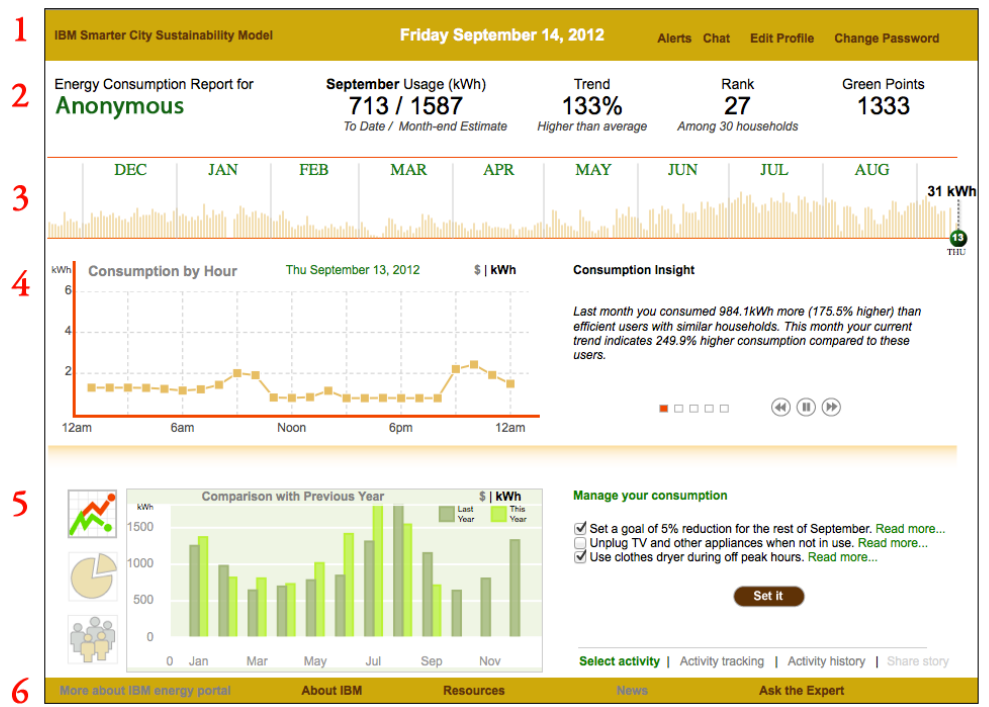
\includegraphics[scale=0.26]{./electricity_portal.png}
	\caption{The electricity portal divided in the 6 bands. \cite{erickson2013dubuque}}
	\label{fig:electricityportal}
\end{figure}

The user interface of the portal can be seen in Figure~\ref{fig:electricityportal}. It is divided into 6 bands:
\begin{enumerate}
\item Header, with date and menu access.
\item User name, usage to date, estimate of current month's usage and three incentives: trend (for self comparison), rank (among other households) and `green points', which can be collected with actions such as completing one's profile.
\item Daily electricity usage displayed in kWh or in dollar.
\item A graph of todays consumption and a textual comparison of the users electricity consumption.
\item A graph allowing users to view their energy usage compared to the previous year, broken down by load or compared to 30 similar households. It also has a component where users can view and set their goals.
\item Links to general information.
\end{enumerate}

The portal was made available to 765 households in a few contiguous neighborhoods in the city of Dubuque in the United States and ran for about 20 weeks. Use of the portal was logged and surveys and interviews were held to find out about the experiences of the users of the portal.


%results
%  numbaahs
%Out of 35\% of households in the study logged into the portal at least one time.
In the survey, respondents were asked to estimate how often they used the portal. The responses were as follows:
\begin{enumerate}
\item five or more times per week -- 12\%
\item about once a week -- 18\%
\item occasional use -- 31\%
\item rare use -- 25\%
\item not applicable / do not recall -- 14\%
\end{enumerate}

In the survey, participants were also asked about the UI components. They were asked whether they usually looked at them, if they needed more explanation, if it helped them to better understand their electricity consumption and if it encouraged them to undertake action. The responses in percentages to these questions can be seen in Table~\ref{uicomponents}.

From these results it can be concluded that the historical consumption (consumption timeline/consumption by hour) are the most popular. Also the component displaying the comparison with own prior use (historical comparison) was used often.
he first four components, which are the most looked at are all time-based graphs/metrics. 

\begin{table}
  \caption{The UI components, ordered by popularity with the answers by participants to questions in percentages}
  \label{uicomponents}
  \scriptsize
  \begin{center}
    \begin{tabular}{lcccc}
    
        & \multicolumn{1}{p{1.2cm}}{\centering Usually looked at it} & 
        \multicolumn{1}{p{1.0cm}}{\centering Was entirely clear} & 
        \multicolumn{1}{p{1.3cm}}{\centering Helped to understand use} & 
        \multicolumn{1}{p{1.2cm}}{\centering Encouraged to act} \\ \hline
        
        \pbox{20cm}{Consumption\\ timeline} & 93\% & 53\% & 76\% & 49\% \\[0.25cm]
        \pbox{20cm}{Consumption\\ by hour} & 87\% & 53\% & 79\% & 52\% \\[0.25cm]
        \pbox{20cm}{Comparison with\\ previous year} & 87\% & 55\% & 58\% & 44\% \\[0.25cm]
        \pbox{20cm}{Monthly usage} & 81\% & 49\% & 58\% & 45\% \\[0.1cm]
        \pbox{20cm}{Consumption\\ insights} & 77\% & 38\% & 46\% & 47\% \\[0.25cm]
        \pbox{20cm}{Comparison \\with neighbor} & 67\% & 33\% & 30\% & 28\% \\[0.25cm]
        \pbox{20cm}{Consumption\\ by load} & 64\% & 40\% & 48\% & 31\% \\[0.20cm]
        \pbox{20cm}{Trend, Rank, Points} & 64\% & 32\% & 41\% & 44\% \\[0.05cm]
        \pbox{20cm}{Manage your\\ consumption} & 62\% & 46\% & 34\% & 35\% \\[0.1cm]
        \pbox{20cm}{Alerts} & 32\% & 33\% & 24\% & 19\% \\
    \end{tabular}
  \end{center}
\end{table}

All 266 participating households reduced their electricity usage. Compared to electricity consumption of the previous year, they saved on average $31,817$ kWh during the project. This amounts to a monthly reduction of 3.7\%. In the survey, 69\% of the respondents indicated that the portal increased their understanding of how they consume electricity.

The study reports that, while the percentage of participants using the goal setting component (``Manage your consumption'') is only 62\%, this group of participants achieved over half of the savings. Their monthly reduction was about 7\%.

\subsection{Results}
The previous parts and the guidelines that some eco-feedbacks systems researches have established allow us to extract some requirements that the UI of eco-feedback should meet in order help the developers implementing software as effective as possible for the users. \\ %AFTER RE REVIEW ADD THIS: In the first subsection "famous" guidelines will be presented and in the second one the list of requirements. 

%DIRECT COMPARISON: TABLE WITH ++ AND -~-~~(summary)
%
%\begin{table}
%  \caption{Overview of the results}
%  \label{table:results}
%  \scriptsize
%  \begin{center}
%    \begin{tabular}{|l|c|}
%       \hline
%       \textbf{UI component} & \textbf{Rating} \\
%       \hline
%       Consumption over time & \\
%       Historical comparison & \\
%       Normative comparison & \\
%       Incentives & \\
%       Disaggregation & \\
%       Goal setting & \\
%       \hline
%    \end{tabular}
%  \end{center}
%\end{table}

\subsubsection{Consumption over time}
The `consumption over time' component is one of the most basic UI components for eco-feedback systems. From the study by S. Karjalainen, we can conclude that it is mostly effective when the consumption is displayed in terms of costs instead of, for example, kWh.

The study by Erickson et al. also showed that this component is the most popular and respondents to their survey indicated that this component contributed the most to understanding their energy usage.
\subsubsection{Historical comparison}
The `historical comparison' component was also very popular. However, as the survey results from Erickson et al. indicate, the component is a lot less insightful to users than the `consumption over time'. 

The components also helps with increased retention, as the study by R. Jain et al. shows that this component leads to more logins of users.
\subsubsection{Normative comparison}
The interest from participants in the study by Karjalainen for the `normative comparison' component was not very high. 
Additionally, the study from Erickson et al. found that the interest from users for this component was also not very high. Users indicated that the component did not provide much helpful information to them to aid them in reducing their electricity consumption. In the survey from Erickson, a lot of respondents said that they ``were uninterested in how they compared to others''.

However, the study from Peschiera et al. has found that the use of normative comparison does aid in saving more energy. This seems to be contradicting with results from the other studies and more research would be required to know more about the effectiveness of this UI component.
\subsubsection{Incentives}
The use of incentives/rewards \& penalization, appears to be effective from the study by R.K. Jain et al., especially when it emphasizes rewards over penalizations. %TODO find other study for incentives

\subsubsection{Disaggregation}
In the study by Karjalainen, one of the components most valued by consumers was the disaggregation component. 

In the study by R.K. Jain et al. however, the presence of the disaggregation component did not lead to more logins. It is mentioned by them that this is not consistent with previous research. 
They reason that this could be due to the fact that the disaggregation component requires a lot of configuration from the user. This can be experienced by users as tedious and users might not be willing to invest such an amount of time into this UI component before being able to use it.

%TODO: future research -> how to make it easier configurable
%A lack of support for the disaggregation component
%is incongruent with recent research [6,11] that suggested users
%who have a deeper understanding of appliance specific consump-
%tion would reduce consumption and login to the interface more
%often

\subsubsection{Goal setting}
For the goal setting, we can conclude from the study by S. Karjalainen that people were not really interested in the goal setting component. However, this UI component does seem very valuable, because in the study by Erickson et al., the group of participants using this UI component achieved over half of the savings.


\section{Discussion}
In this comparative paper, the effects of the UI components in several studies are used. These studies have all taken place in different environments and during different times which makes it difficult to compare the obtained results.

The results obtained from the studies about the normative comparison are contradicting. Some studies indicate that users are not interested in this component and that it is not helpful to them, whereas other the study by Peschiera et al. obtained results that suggest that the normative UI component leads to significantly more energy savings.

%blended normative / incentives
Also, the study from Erickson et al. combines the UI component for incentives with a normative comparison. They reward energy saving behavior with points (which is a reward), but also user the numbers of points the user collects in a ranking, which compares all the users.\\

%TODO: Blabla about the interview.\\
% Why did we make this interview
%We conducted this interview in order to have more ifnormation about somone who have experienced in the deisgn of ECF in different fields, different users, to have a broader insight/view
% Although there is no perfect answer, it soesnt prevail over what we said before (bias etc) having the opinion of an expert gave us information that we didn't find in the litterature, it raised some issues that we didn't imagine before
% confirmer or invalidate what we read before, add information about his experience , sees if a agrees of disagrees with what was said before etc

%During an interview we conducted with an expert of the field, he shared his experience and gave us more information about the design of ECF systems.
%As we saw in the previous parts, some design components are more likely to help the users in understanding their electricity usage.
%However, depending on the demand and the location where the UI will be displayed there are some differences, as the researcher said: ``You do not display the same thing in an art faculty and in a science faculty''.

There are no universal rules when it comes to the design of eco-feedback systems systems. The design is also influenced by external factors, such as the environment, background/education of the users and goal of the system: saving money or taking care of the environment.
For example, some building managers will not allow visitors of the building to see how much money is spent on the electricity used. The designers have to take the client requirements into account.
% Do we say something about colors??



%\section{Recommendations for UI designer}
%
%
%\subsection {List of requirements}
%
%The results from the surveys and the interview allow us to establish a list of requirements that must/should be fulfilled by the designers in order to build ECF systems as effective as possible:
%
%%TODO: add the source karjalainen
%
%Sustainability and long term-commitment
%Non-intrusiveness and Acceptability
%Learnability and Intuitiveness
%Usability
%Actionable

% guidelines of the guy

\section{Conclusion}
In this paper, we looked at different user interface components used in eco-feedback systems. Based on several studies, we conclude that problems with understanding these interfaces for consumers are often caused by unfamiliarity with the scientific units used or how CO$_2$ relates to electricity usage. \\

Out of several studies, it can be concluded that interface components that present information in charts and tables are easily understood by consumers, especially when they concern time-based graphs/metrics. \\

From the researched studies, we can conclude that the `consumption over time' and `historical comparison' UI components are generally the most popular and most insightful, especially when consumption is displayed in terms of costs.

The `goal setting' component leads to a very significant increase in energy usage. However, the interest from users is generally low. When this component is used, it is therefore important to promote the use of it by users of the eco-feedback system.

Disaggregation is valued highly by users of eco-feedback systems. It provides a lot of insightful and actionable information. However, a larger time to configure this component correctly, means that it is sometimes not used by consumers. This should be kept in mind when using this component in an eco-feedback system.

The use of incentives to motivate consumers to save electricity is also effective in making consumers use the eco-feedback system, especially when users of the system start with a positive number of points.

The comparison for the `normative comparison'  UI component is inconclusive and requires further research to study its effectiveness.
%It can also be concluded that using electricity usage information from peer networks can lead to more consistent energy saving when compared to only showing the users own electricity usage.

% OMG , PUT THIS IN HEREE: we also see a trend -> components that are not popular (large config time or uninterested [goal setting]) are often very effective.
% we recoommend to promote/highlight these components and aid user with configuration to get significant benefit for energy saving

\section{Future work}
% normative comparison
% we are not sure yet about what is the 'best' display, it depends on the users and the place
Our comparative analysis showed that more research is needed to find out when the normative comparison UI component is effective and how users can be motivated to use this component.

We also saw that the goal setting is very effective, but not very popular with users. It can be helpful for UI designers of eco-feedback system if more research will be available about why the goal setting component is so unpopular and how users can be motivated to use this component.

In this comparative paper, we did not look at how interaction between users and eco-feedback systems can aid in saving more energy and this can be interesting for future work, since interaction is an important part of the interface between the system and the user.

We also did not talk about more subtle things in the UI like the use of colors (in e.g. the charts) and we did not get to a result for which device is the most appropriate, as this most likely differs per targeted user group.

%% if specified like this the section will be ommitted in review mode
\acknowledgements{
The authors wish to thank S. Cretu and M. Medema for their feedback and also I. Georgievski for his expert review and answers to questions.}

\bibliographystyle{abbrv}
%%use following if all content of bibtex file should be shown
%\nocite{*}
\bibliography{template}
\end{document}
